\documentclass[a4paper]{article}
\setlength{\topmargin}{-1.0in}
\setlength{\oddsidemargin}{-0.2in}
\setlength{\evensidemargin}{0in}
\setlength{\textheight}{10.5in}
\setlength{\textwidth}{6.5in}
\usepackage{enumitem}
\usepackage{amsmath}
\usepackage{hyperref}
\usepackage{amssymb}
\usepackage[dvipsnames] {xcolor}
\usepackage{mathpartir}
\usepackage{graphicx}

\hbadness=10000

\hypersetup{
    colorlinks=true,
    linkcolor=blue,
    filecolor=magenta,      
    urlcolor=cyan,
    pdftitle={Assignment 2},
    pdfpagemode=FullScreen,
    }
\def\endproofmark{$\Box$}
\newenvironment{proof}{\par{\bf Proof}:}{\endproofmark\smallskip}
\begin{document}
\begin{center}
{\large \bf \color{red}  Department of Computer Science} \\
{\large \bf \color{red}  Ashoka University} \\

\vspace{0.1in}

{\large \bf \color{blue}  Introdution to Quantitative Finance}

\vspace{0.05in}

    { \bf \color{YellowOrange} Assignment 1}
\end{center}
\medskip

\hfill {\textbf{Name: Rushil Gupta} }

\bigskip
\hrule


% Begin your assignment here %

\section*{Question 1}
\begin{enumerate}
    \item \begin{enumerate}[label=(\alph*)]
        \item We initially have a principal amount of $P_0$. Since the interest is compounded $n$ times annually, the interest rate per compounding period is $\frac{r}{n}$. Now, the first time we recieve an interest, we get:\\
        
        \[ P_1 = P_0 \cdot (1 + \frac{r}{n}) \]

        Now, the second time we recieve an interest, we get:

        \[ P_2 = P_1 \cdot (1 + \frac{r}{n}) = P_0 \cdot (1 + \frac{r}{n}) \cdot (1 + \frac{r}{n}) = P_0 \cdot (1 + \frac{r}{n})^2 \]

        We know that we compound $n$ times each year for $t$ years. So, in total, we have $n \cdot t$ compounding periods. So, the final amount we get is:

        \[ P_{nt} = P_0 \cdot (1 + \frac{r}{n})^{nt} \]

        \vspace{15mm}

        \item The graph below shows the variation of $P_{n \cdot t}$ with $n \in [1, 10000] \land (100 \mid n)$.
        \begin{figure}[h]
            \centering
            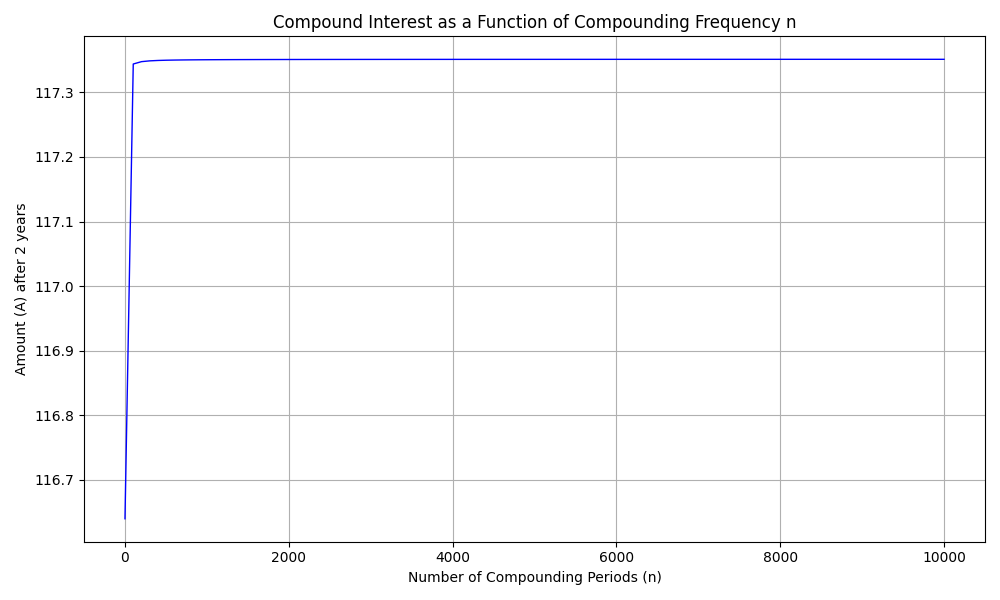
\includegraphics[width=0.85\textwidth]{Q1.png}
            \caption{Graph of $P_{n \cdot t}$ vs $n$}
        \end{figure}

        \vspace{15mm}

        \item The plot shows that as you compound more times an year, the higher overall return you get. This is an intuitive result because the interest rate is divided by a factor of $n$, but is inturn raised to the power of $n$, leading to the higher returns. However, in the plot above, it is clear that the returns start to saturate after a certain point, and they flatline for $n \geq 500$ (approx).
        
        \newpage
        
        \item Currently, we have the expression for $P_{nt}$ as:
        \[ P_{nt} = P_0 \cdot (1 + \frac{r}{n})^{nt} \]

        Taking the limit of $n \rightarrow \infty$, we get:
        \[ P_0 \cdot \lim_{n \to \infty} (1 + \frac{r}{n})^{nt} \]
        \[ = P_0 \cdot \lim_{n \to \infty} ((1 + \frac{r}{n})^{n})^t \]
        \[ = P_0 \cdot (\lim_{n \to \infty} (1 + \frac{r}{n})^{n})^t \]

        We know that $\lim_{n \to \infty} (1 + \frac{r}{n})^{n} = e^r$. So, the final expression is:
        \[ P_{\infty} = P_0 \cdot (e^r)^t = P_0 \cdot e^{rt} \]
    \end{enumerate}

    \vspace{15mm}
    \section*{Question 2}
    \item \begin{enumerate}
        \item We can find which scheme is better to buy the house by finding the net present value of both the schemes. \\
        
        Scheme 1: \\
        \[ V_1 = \frac{70 + 6}{1 + 0.1} + \frac{70 + 8}{(1 + 0.1)^2} + \frac{70 + 10}{(1 + 0.1)^3} \]
        \[ = \frac{76}{1.1} + \frac{78}{1.21} + \frac{80}{1.331} \]
        \[ = 193.66 \]

        Scheme 2: \\
        \[ V_2 = \frac{50 + 6}{1 + 0.1} + \frac{50 + 8}{(1 + 0.1)^2} + \frac{50 + 10}{(1 + 0.1)^3} + \frac{50 + 13}{(1 + 0.1)^4} \]
        \[ = \frac{56}{1.1} + \frac{58}{1.21} + \frac{60}{1.331} + \frac{63}{1.4641} \]
        \[ = 186.95 \]

        Since we want to buy the house, we should choose the scheme with the lower net present value. Hence, scheme 2 is better.

        \vspace*{15mm} 

        \item We know that the corpus will be required once the apartment is bought. We also know that Rs. 2 lakhs will be withdrawn each year. So, the corpus should be able to sustain this withdrawal for an infinite amount of time, given the interest rate of 10\%. So, the corpus should be:
        \[ M = \frac{2}{0.1} = 20 \]

        Hence, the maintenance corpus should be Rs. 20 lakhs.

        \vspace*{15mm}
        \item After taking into consideration the maintenance corpus, the net present value of the schemes will change. We will need to add the net present value of the corpus adjusted by the year the apartment is bough to the current net present values we have. \\
        
        \[ V_1 = V_1 + \frac{20}{1.1^3} = 193.66 + 15.02 = 208.68 \]

        \[ V_2 = V_2 + \frac{20}{1.1^4} = 186.95 + 13.56 = 200.61 \]

        Scheme 2 is better as it has a lower net present value. Hence, the decision between the two schemes will not change.
    \end{enumerate}
    
    \vspace*{15mm}
    \section*{Question 3}
    \item \begin{enumerate}
        \item Project 1: \\
        \[ NPV_1 = -100 + \sum_{i=1}^{5} \frac{30}{(1 + 0.1)^i} = 13.72 \text{ lakhs}\]
        \[ 0 = -100 + \sum_{i=1}^{5} \frac{30}{(1 + IRR_1)^i} \implies IRR_1 = 15.23\%\]

        Project 2: \\
        \[ NPV_2 = -150 + \sum_{i=1}^{5} \frac{42}{(1 + 0.1)^i} = 9.21 \text{ lakhs}\]
        \[ 0 = -150 + \sum_{i=1}^{5} \frac{42}{(1 + IRR_2)^i} \implies IRR_2 = 12.38\%\]

        \vspace*{15mm}
        \item Clearly, project 1 has a higher net present value and a higher internal rate of return. Hence, project 1 makes more sense economically as it has a higher return on investment and is more profitable.
    \end{enumerate}

    \newpage
    \section*{Question 4}
    \item \begin{enumerate}
        \item The returns of the mutual funds each year are:
        \[ R_1 = \frac{30 - 25}{25} = 0.2 \]
        \[ R_2 = \frac{32 - 30}{30} = \frac{1}{15} \]
        \[ R_3 = \frac{37 - 32}{32} = \frac{5}{32} \]
        \[ R_4 = \frac{40 - 37}{37} = \frac{3}{37} \]
        \[ R_5 = \frac{41 - 40}{40} = \frac{1}{40} \]
        
        \vspace{3mm}
        The nominal average return for mutual funds is:
        \[ \text{Average Return} = 100 \cdot \frac{0.2 + \frac{1}{15} + \frac{5}{32} + \frac{3}{37} + \frac{1}{40}}{5} = 10.58\% \]

        \vspace{10mm}
        The returns of the treasury bills each year are:
        \[ R_1 = \frac{27 - 25}{25} = 0.08 \]
        \[ R_2 = \frac{29 - 27}{27} = \frac{2}{27} \]
        \[ R_3 = \frac{31 - 29}{29} = \frac{2}{29} \]
        \[ R_4 = \frac{34 - 31}{31} = \frac{3}{31} \]
        \[ R_5 = \frac{36 - 34}{34} = \frac{1}{17} \]

        \vspace{3mm}
        The nominal average return for treasury bills is:
        \[ \text{Average Return} = 100 \cdot \frac{0.08 + \frac{2}{27} + \frac{2}{29} + \frac{3}{31} + \frac{1}{17}}{5} = 7.57\% \]

        \vspace{15mm}
        \item The nominal internal rate of is given by:
        \[ 0 = R_0 + \sum_{i=1}^{5} \frac{R_i}{(1 + IRR)^i} \] \\

        For the mutual fund, we invest 25 and get 41 after 5 years. So, the IRR for mutual funds is:
        \[ 0 = -25 + \frac{41}{(1 + IRR)^5} \implies IRR = 10.40\% \] \\

        Similarly, for the treasury bills, we invest 25 and get 36 after 5 years. So, the IRR is:
        \[ 0 = -25 + \frac{36}{(1 + IRR)^5} \implies IRR = 7.57\% \]

        \newpage
        \item Table 4:

        \begin{tabular}{|c|c|c|c|c|c|}
            \hline
            \multicolumn{2}{|c|}{} & \multicolumn{2}{|c|}{Mutual Funds} & \multicolumn{2}{c|}{Treasury Bills} \\
            \hline
            Year & Inflation & Nominal Return & Real Return & Nominal Return & Real Return \\
            \hline
            1 & 5\% & 20.00\% & 14.29\% & 8.00\% & 2.86\% \\
            \hline
            2 & 5\% & 6.67\% & 1.59\% & 7.41\% & 2.30\% \\
            \hline
            3 & 5\% & 15.63\% & 10.12\% & 6.90\% & 1.81\% \\
            \hline
            4 & 4\% & 8.11\% & 3.95\% & 9.68\% & 5.46\% \\
            \hline
            5 & 4\% & 2.50\% & -1.44\% & 5.88\% & 1.81\% \\
            \hline
        \end{tabular}

        \vspace{5mm}
        Table 5:

        \begin{tabular}{|c|c|c|c|c|}
            \hline
            Year & Inflation Premium & Real Risk-Free Return & Risk Premium \\
            \hline
            1 & 5\% & 2.86\% & 12.00\% \\
            \hline
            2 & 5\% & 2.30\% & -0.74\% \\
            \hline
            3 & 5\% & 1.81\% & 8.73\% \\
            \hline
            4 & 4\% & 5.46\% & -1.56\% \\
            \hline
            5 & 4\% & 1.81\% & -3.38\% \\
            \hline
        \end{tabular}
    \end{enumerate}

    \vspace{15mm}
    \section*{Question 5}
    \item \begin{enumerate}
        \item Cash Flows for Water Purifier A:
        \begin{align*}
            \text{Year 0:} & \quad -2000 \quad (\text{initial purchase}) \\
            \text{Year 1:} & \quad -100 \quad (\text{maintenance}) \\
            \text{Year 2:} & \quad -100 + 50 \quad (\text{maintenance + salvage}) \\
            \text{Year 2:} & \quad -2000 \quad (\text{second purchase}) \\
            \text{Year 3:} & \quad -100 \quad (\text{maintenance}) \\
            \text{Year 4:} & \quad -100 + 50 \quad (\text{maintenance + salvage})
        \end{align*}
        
        NPV for A:
        \[
        NPV_A = -2000 - \frac{100}{1.1} - \frac{100 + 50}{1.1^2} - \frac{2000}{1.1^2} - \frac{100}{1.1^3} - \frac{100 + 50}{1.1^4} = -3894.41
        \]
        
        \vspace{5mm}
        Cash Flows for Water Purifier B:
        \begin{align*}
            \text{Year 0:} & \quad -3000 \quad (\text{initial purchase}) \\
            \text{Year 1:} & \quad -200 \quad (\text{maintenance}) \\
            \text{Year 2:} & \quad -200 \quad (\text{maintenance}) \\
            \text{Year 3:} & \quad -200 \quad (\text{maintenance}) \\
            \text{Year 4:} & \quad -200 + 75 \quad (\text{maintenance + salvage})
        \end{align*}
        
        NPV for B:
        \[
        NPV_B = -3000 - \frac{200}{1.1} - \frac{200}{1.1^2} - \frac{200}{1.1^3} - \frac{200 + 75}{1.1^4} = -3582.75
        \]

        Clearly, Water Purifier B is the better choice as it has a higher NPV, which in this case is the same as saying a lower absolute NPV (since we want to minimize the cost).


        \vspace{15mm}
        \item Cash Flows for Water Purifier A:
        \begin{align*}
            \text{Year 0:} & \quad -2000 \quad (\text{initial purchase}) \\
            \text{Year 1:} & \quad -100 \quad (\text{maintenance}) \\
            \text{Year 2:} & \quad -100 + 50 \quad (\text{maintenance + salvage}) \\
            \text{Year 3:} & \quad -2000 \quad (\text{second purchase}) \\
            \text{Year 4:} & \quad -100 \quad (\text{maintenance}) \\
            \text{Year 5:} & \quad -100 + 50 \quad (\text{maintenance + salvage}) \\
            \text{Year 6:} & \quad -2000 \quad (\text{third purchase}) \\
            \text{Year 7:} & \quad -100 \quad (\text{maintenance}) \\
            \text{Year 8:} & \quad -100 + 50 \quad (\text{maintenance + salvage})
        \end{align*}
                
        NPV for A over 6 years:
        \[
        NPV_{A_{6yrs}} = -5350.75
        \]
        
        \vspace{5mm}
        Cash Flows for Water Purifier B:
        \begin{align*}
            \text{Year 0:} & \quad -3000 \quad (\text{initial purchase}) \\
            \text{Year 1:} & \quad -200 \quad (\text{maintenance}) \\
            \text{Year 2:} & \quad -200 \quad (\text{maintenance}) \\
            \text{Year 3:} & \quad -200 + 75 \quad (\text{maintenance + salvage}) \\
            \text{Year 4:} & \quad -3000 \quad (\text{second purchase}) \\
            \text{Year 5:} & \quad -200 \quad (\text{maintenance}) \\
            \text{Year 6:} & \quad -200 + 75 \quad (\text{maintenance + salvage})
        \end{align*}

        NPV for B over 6 years:
        \[
        NPV_{B_{6yrs}} = -6026.31
        \]

        In this case, Water Purifier A is the better choice as it has a higher NPV, which in this case is the same as saying a lower absolute NPV (since we want to minimize the cost).
    \end{enumerate}


    \vspace{15mm}
    \section*{Question 6}
    \item \begin{enumerate}
        \item We first begin by calculating the yeild of the two bonds. \\

        For the 9\% coupon bond, the yield is:
        \[ 101 = \sum_{i=1}^{5}{\frac{9}{(1 + \lambda_1)^i}} + \frac{100}{(1 + \lambda_1)^5} \implies \lambda_1 = 8.745\% \]

        For the 7\% coupon bond, the yield is:
        \[ 93.20 = \sum_{i=1}^{5}{\frac{7}{(1 + \lambda_2)^i}} + \frac{100}{(1 + \lambda_2)^5} \implies \lambda_2 = 8.736\% \]

        This means the average yield of the two bonds is $8.74\%$. So, the price of a 5-year zero coupon bond is:
        \[ P = \frac{100}{(1 + 0.0874)^5} = 65.77 \]


        \newpage
        % b) Suppose the 4-year spot rate is 3.4%. What is the 1-year forward rate between years 4 and 5?
        \item We know that the 4-year spot rate is 3.4\%. So, the price of a 4-year zero can be found through the following equation:

        \[ (1 + s_5)^5 = (1 + s_4)^4 \cdot (1 + f_{4,5}) \]

        Since we know the yeild of the 5-year zero coupon bond, we can use it as the spot rate for the 5th year. So, the equation becomes:

        \[ (1 + 0.0874)^5 = (1 + 0.034)^4 \cdot (1 + f_{4,5}) \]
        \[ \implies f_{4, 5} = \frac{(1 + 0.0874)^5}{(1 + 0.034)^4} - 1 = 0.330 \]

        Hence, the 1-year forward rate between years 4 and 5 is 33.0\%.
    \end{enumerate}

    \vspace*{15mm}
    \section*{Question 7}
    \item REDACTED


    \vspace*{15mm}
    \section*{Question 8}
    \item We can immunize our portfolio by ensuring that the duration of the portfolio is equal to the duration of the liability, and make sure we invest a total of 10 lakhs in the two bonds. \\
    
    For this, we first find the price (= present value) of the two bonds.

    \[ P_A = \sum_{i=1}^{3} \frac{20000}{(1 + 0.05)^i} + \frac{500000}{(1 + 0.05)^3} = 486383.76 \]
    \[ P_B = \sum_{i=1}^{7} \frac{30000}{(1 + 0.05)^i} + \frac{500000}{(1 + 0.05)^7} = 528931.87 \]

    Now, we find the duration of the two bonds.

    \[ D_A = \frac{\left( \sum_{i=1}^{3} \frac{i \cdot 20000}{(1 + 0.05)^i} + \frac{3 \cdot 500000}{(1 + 0.05)^3} \right)}{P_A} = 2.88 \text{ years} \]
    \[ D_B = \frac{\left( \sum_{i=1}^{7} \frac{i \cdot 30000}{(1 + 0.05)^i} + \frac{7 \cdot 500000}{(1 + 0.05)^7} \right)}{P_B} = 5.95 \text{ years} \]
    
    Let $V_1 = 486383.76x$ and $V_2 = 528931.87y$ be the amount invested in Bond A and Bond B respectively. Finally, this gives us the following linear equations:
    
    \[ V_1 + V_2 = 1000000 \]
    \[ 2.88V_1 + 5.95V_2 = 5 \cdot 1000000 \]


    Solving these equations, we get $V_1 = 310226$ and $V_2 = 689774$ (rounded off to the nearest integer). This means we buy $V_1$ worth of Bond A and $V_2$ worth of Bond B to immunize our portfolio.

    \newpage

    Now, considering the situation that there is a 1\% interest rate hike, we can calculate the new prices and duration of the bonds. \\

    \begin{align*}
        P'_A &= \sum_{i=1}^{3} \frac{20,000}{(1.06)^i} + \frac{500,000}{(1.06)^3} = 473,269.88 \\
        P'_B &= \sum_{i=1}^{7} \frac{30,000}{(1.06)^i} + \frac{500,000}{(1.06)^7} = 500,000.00 \\
        D'_A &= \frac{\sum_{i=1}^{3} \frac{i \cdot 20,000}{(1.06)^i} + 3 \cdot \frac{500,000}{(1.06)^3}}{P_A^{new}} = 2.88 \\
        D'_B &= \frac{\sum_{i=1}^{7} \frac{i \cdot 30,000}{(1.06)^i} + 7 \cdot \frac{500,000}{(1.06)^7}}{P_B^{new}} = 5.92
    \end{align*}

    We put the same value in each bond as before, and calculate the new portfolio value and duration. The total portfolio size would be the same since we did not change the amount invested in each bond.

    \begin{align*}
        \text{Total Portfolio Duration (New)} &= \frac{2.88V_1 + 5.92V_2}{1000000} = 4.98 \text{ years} \\
    \end{align*}

    Since the duration of the portfolio is not equal to the duration of the liability, the portfolio is not perfectly immune to changes in the impending obligation. However, the portfolio is still quite immune to changes in the interest rate. Moreover, even with the 1\% interest rate hike, the portfolio will still be able to pay of the liability.



\end{enumerate}
\end{document}A1/Assignment1.tex